\documentclass[journal, a4paper]{IEEEtran}
\usepackage{verbatim} 
\usepackage{booktabs}
\usepackage{multirow}
\usepackage[table,xcdraw]{xcolor}
\usepackage[export]{adjustbox}
\usepackage{graphicx}
\usepackage{adjustbox} 
\usepackage{url}
\usepackage{hyperref}
\usepackage{caption}
\usepackage{subcaption}
\usepackage{amsmath} 
\usepackage{enumitem}
\usepackage{cite}      
\usepackage{graphicx}   
\usepackage{psfrag}   
\usepackage{stfloats}  
\usepackage{amsmath}    
\interdisplaylinepenalty=2500                
\usepackage{array}
\usepackage{hyperref}
\usepackage{tabularx}


\title{Video Surveillance for Road Traffic Monitoring}

  \author{
  Caballero, Ana 
  \texttt{ana.caballeroc@e-campus.uab.cat}
  \\[1ex]
  Vallve, Arnau 
  \texttt{arnau.vallve@e-campus.uab.cat}
  \\[1ex]
  Malak, Marcin 
  \texttt{malak.marcin@e-campus.uab.cat}
  \\[1ex]
  Jaworski, Wiktor 
  \texttt{jaworski.wiktor@e-campus.uab.cat}
  
  \thanks{Under the guidance of  ~Javier Ruiz and ~Xavier Giro.}
}
\date{April 2019}

%\address{Universidad Politècnica de Catalunya, Barcelona, España\\}

\begin{document}


\markboth{Machine Learning for Computer Vision}{}
\maketitle


\begin{abstract}

This work proposes a framework to learn  the basic concepts and techniques related to video sequences mainly for surveillance applications and can be applied to any problem in order to obtain accurate automatic results. The system is based on the NVIDIA AI CITY Challenge \cite{Nvidia}. We started with a foreground estimation, then post processing techniques are applied to the detect and track vehicles in motion. Finally, we stabilized video with Optical Flow and applied all we learned to multiple cameras. The project has been developed in Python \cite{GitRepo}. However, this report is focused just in the last week of the work.

\end{abstract}

\section{Introduction}
\label{sec:Introduction}
\IEEEPARstart{T}{he}
 use of intelligent traffic surveillance systems, based on algorithms and computer vision systems are very useful at present to improve the problems of traffic congestion and any anomaly that may occur on the roads such as accidents or dangerous infractions. These systems, based on numerical data, process the information received through the network of video cameras already used for a long time to check traffic on the roads and extract information in real time for operators to process and collect statistics to improve traffic flows. traffic.\\
 
These systems are essential in our times due to the great increase in traffic and the human difficulty of processing so much information in real time and giving an immediate response to solve the problem.

\section{The NVIDIA AI CITY CHALLENGE}
\label{sec:NVidia}
The aim of this challenge is to encourage the research and development techniques that rely less on supervised approaches and more on transfer learning, unsupervised and semi-supervised approaches that go beyond bounding boxes.  It is focused on \textbf{Intelligent Transportation System (ITS)} to  satisfy the need of  making transportation systems smarter. \\

Nvidia proposes three challenges with different datasets provided as a set of videos or images, as images in figure \ref{fig:nvidiaImages}. These challenges are: 

\begin{itemize}
\item City-scale multi-camera vehicle tracking
\item City-scale multi-camera vehicle re-identification
\item Traffic anomaly detection 
\end{itemize}

Out project is focused on the first track challenge:  \textbf{City-scale multi-camera vehicle tracking}.

%%%%%%%%%% IMAGES %%%%%%%%%%%%%
\begin{figure}[ht] \centering
\begin{subfigure}[b]{0.22\textwidth}
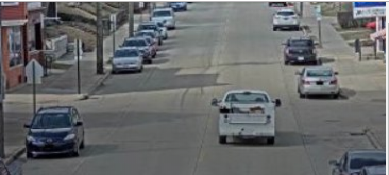
\includegraphics[scale=.5]{images/nvidia1.png}   
\subcaption{\label{fig:nvidia1png} Image frame example 1}
\end{subfigure}
\hspace{0.2cm}
\begin{subfigure}[b]{0.22\textwidth}
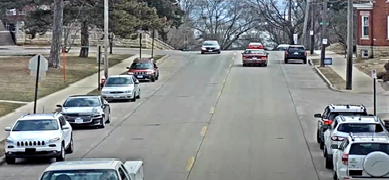
\includegraphics[scale=.5]{images/nvidia2.png}   
\subcaption{\label{fig:nvidia2png} Image frame example 2}
\end{subfigure}
\caption{\label{fig:nvidiaImages} Example images from Nvidia AI City Challenge web}
\end{figure}
%%%%%%%%%% IMAGES (end) %%%%%%%%%%%%%

\section{MULTI-TARGET SINGLE-CAMERA TRACKING (MTSC)}
\label{sec:MTSC}
There are various solution which allow us to implement multi-target single-camera tracking. For the needs of the subject we tried to implement one of provided and suggested solution:
\begin{itemize}
\item \textbf{Tracking by overlap}
\item \textbf{Kalman filtering}
\end{itemize}
For the first idea, we have been using the concept of adding for each detected car new ID. We have already created for that two different model of BoundingBox and Frame which store data necessary to creating detection for provided video(a). After implementing everything, we figure it out that using very big IoU threshold (0.95) is not working properly(b), because detections with IoU < 0.95 are seen and labeled as new detections. Non in-depth qualitative tests suggest the IoU threshold values close to 0.5 give the best results. High values of look-back frames give bad results for dynamic objects and way better results for non-moving objects. The two parameters could be tweaked to bring the best results for given scenario.
%%%%%%%%%% IMAGES %%%%%%%%%%%%%

\begin{figure}[ht] \centering
\begin{subfigure}[b]{0.22\textwidth}
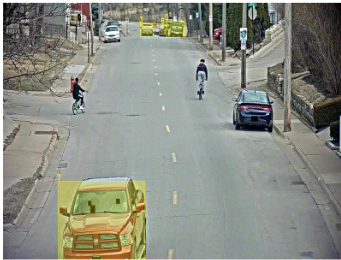
\includegraphics[scale=.7]{images/img1.PNG}   
\subcaption{\label{fig:img1png} Overlap example 1}
\end{subfigure}
\hspace{0.2cm}
\begin{subfigure}[b]{0.22\textwidth}
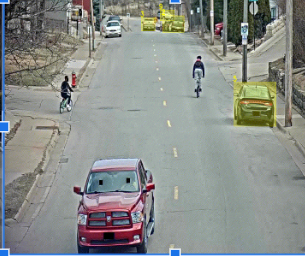
\includegraphics[scale=.7]{images/img2.PNG}   
\subcaption{\label{fig:img2png} Overlap example 2}
\end{subfigure}
\end{figure}

%%%%%%%%%% IMAGES (end) %%%%%%%%%%%%%

As a second approach we tried to implement Kalman filtering. We end up in the situation where prediction is slightly good, but in some particular cases there are mistakes of prediction. 
We are considering that this problem might occur because of the linear nature of the filter. There are different type of movement of cars, not always in linear way. 

We also had some difficulties to find out the reason why our filter in some part of detection changes “bbox id” for other one (which we think it proves that filter is missing detection)

%%%%%%%%%% IMAGES %%%%%%%%%%%%%
\begin{figure}[ht] \centering
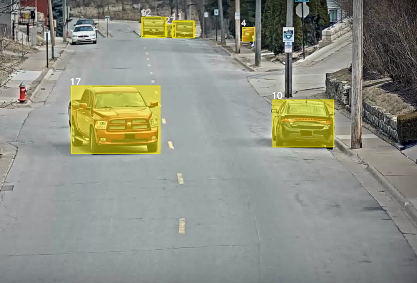
\includegraphics[scale=0.9]{images/img3.PNG}   
\caption{\label{fig:img3} Kalman filtering}
\end{figure}
%%%%%%%%%% IMAGES (end) %%%%%%%%%%%%%

Both of the situation described above occur mostly with the strange and not sufficient results. With all the metrics we have been trying to achieve, we get a strange results. Very different results than expected.

The table below show up the results of metrics we achieved: 

%%%%%%%%%% IMAGES %%%%%%%%%%%%%
\begin{figure}[ht] \centering
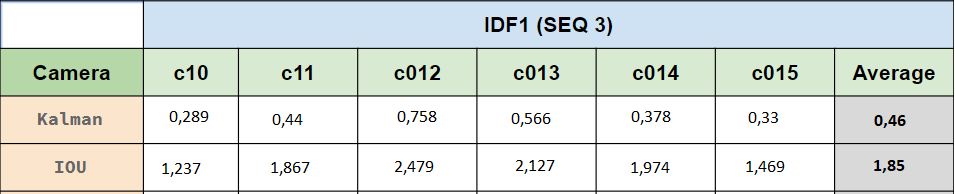
\includegraphics[scale=0.45]{images/img4.png}   
\caption{\label{fig:img4} Results table}
\end{figure}
%%%%%%%%%% IMAGES (end) %%%%%%%%%%%%%




\section{MTSC AND TRACKING BY OVERLAP}
\label{sec:MTSC_Overlap}
Multiple target single camera tracking is the city environment is a very challenging task. It is because of dynamic environment and many possible occlusions that often lead to many errors such as swapping IDs of the objects when occluding. In our case we tried to keep track of each object using \textbf{Kalman filter} or \textit{Overlap tracking}. As seen in \autoref{fig:dadRes} the performance of the the methods was drastically different. Kalman tracking uses the propablisitic methods to assign the same object ID between various frames (from the point of view of Kalman filter - states) to each detected object. For each detection the ID is assigned based on the given error covariance of the prediction. The Overlap simply calcualtes the intersection over union metric between each detection of two frames. The ID is propagated from previous frame to next frame based on the higher IoU score. In our implementation of tracking using IoU we experienced problems when new objects were appearing and that led to bad results. We also tested qualitatively the threshold values (that is minimum IoU to assign the existing ID to an object) and we obtained the best results for values near \textit{0.4}.  Kalman provided results more stable but still we experienced many re-detections - that is perceiving the occluded object in the consecutive frames as new detection and assigning new ID to it.

\section{MULTI-TARGET MULTI-CAMERA TRACKING (MCMT)}
\label{sec:MTMC}
Multi target multi camera tracking was the final goal of the projects. To achieve it we need to:
\begin{itemize}
    \item Detect objects - that is done by fine-tuned off-the shelf object detection system model \textbf{yolov3}
    \item Track targets - done as mentioned in chapter \autoref{sec:MTSC_Overlap}
    \item Re-identify targets, using methods mentioned in chapter \autoref{sec:MTM_Hough_Homog} or using existing systems for car re-identification such as veri-776
    \item Assign the same ID to targets across multiple cameras.
\end{itemize}

\section{MCMT ROBUST HOUGH-BASED HOMOGRAPY PROJECTIONS}
\label{sec:MTM_Hough_Homog}
One of the first approaches we tried in order to work on the multi-camera domain was based on the paper Multi-camera Multi-object Tracking by Robust Hough-based Homography Projections \cite{sternig2011multi} for which no implementation was found, so we tried to implement it by ourselves. The method uses a generalized Hough voting and extends it into a multi-camera domain which is what we require for our problem. This method has the advantage that requires a low amount of data for the voting procedure, it is robust to projection errors and utilizes geometric information to improve the performance of the tracking.

The method revolves around the use of the Hough transform. As the Hough transform allows to find certain shapes on an image using a voting procedure it seems suitable for the task of finding object candidates. However, this method uses a new voting scheme for which the voting results are fused over the multiple cameras. Additionally it also uses geometric verification and backprojection between views to improve the tracking and applies a particle filtering approach to avoid overlapping particles.  

The method can be visually understood by looking at figure \ref{fig:hough}. While most methods based on background subtraction can have projection errors and ghosting detections, the Hough multi-camera voting approach generates Hough maps from voting in each of the cameras we have, which are then projected into a common ground plane where the geometric uncertainties are implicitly considered.

The blocks required in order to make it work are the following. First, a detector must be used in order to obtain the objects we need to track. From there it is required to map the obtained votes from each of the camera views on the common ground plane using the homographies he obtain between the camera and the ground plane. For the voting Hough Forest learning should be used, and the Hough maps should consider voting foot-points instead of the typically used centroids. For the tracking, we want to use multi-object particle filtering with the prior that we don't want objects to occlude in the general plane.

After getting to understand the intricacies of the method and starting to see the issues arising when implementing it from scratch, due to time constraints, it was not possible to evaluate it with our data and implement it for our project. Several alternatives were then also considered.

%%%%%%%%%% IMAGES %%%%%%%%%%%%%
\begin{figure}[ht] \centering
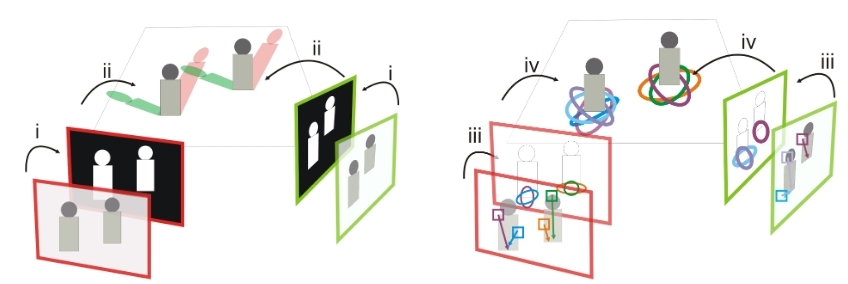
\includegraphics[scale=0.25]{images/hough.jpg}   
\caption{\label{fig:hough} Approach based on background subtraction (left) vs Hough multi-camera by joint votes \cite{sternig2011multi} (right)}
\end{figure}
%%%%%%%%%% IMAGES (end) %%%%%%%%%%%%%

\section{FEATURES FOR MCMT AND RE-IDENTIFICATION}
\label{sec:MTMC_ReID}
DukeMTMC (Duke Multi-Target, Multi-Camera Tracking Project) aims to accelerate advances in multi-target multi-camera tracking. It provides a tracking system that works within and across different cameras, as in figure\ref{fig:duke}, and a new performance evaluation method that measures how often a system is correct about who is where. \\

%%%%%%%%%% IMAGES %%%%%%%%%%%%%
\begin{figure}[ht] \centering
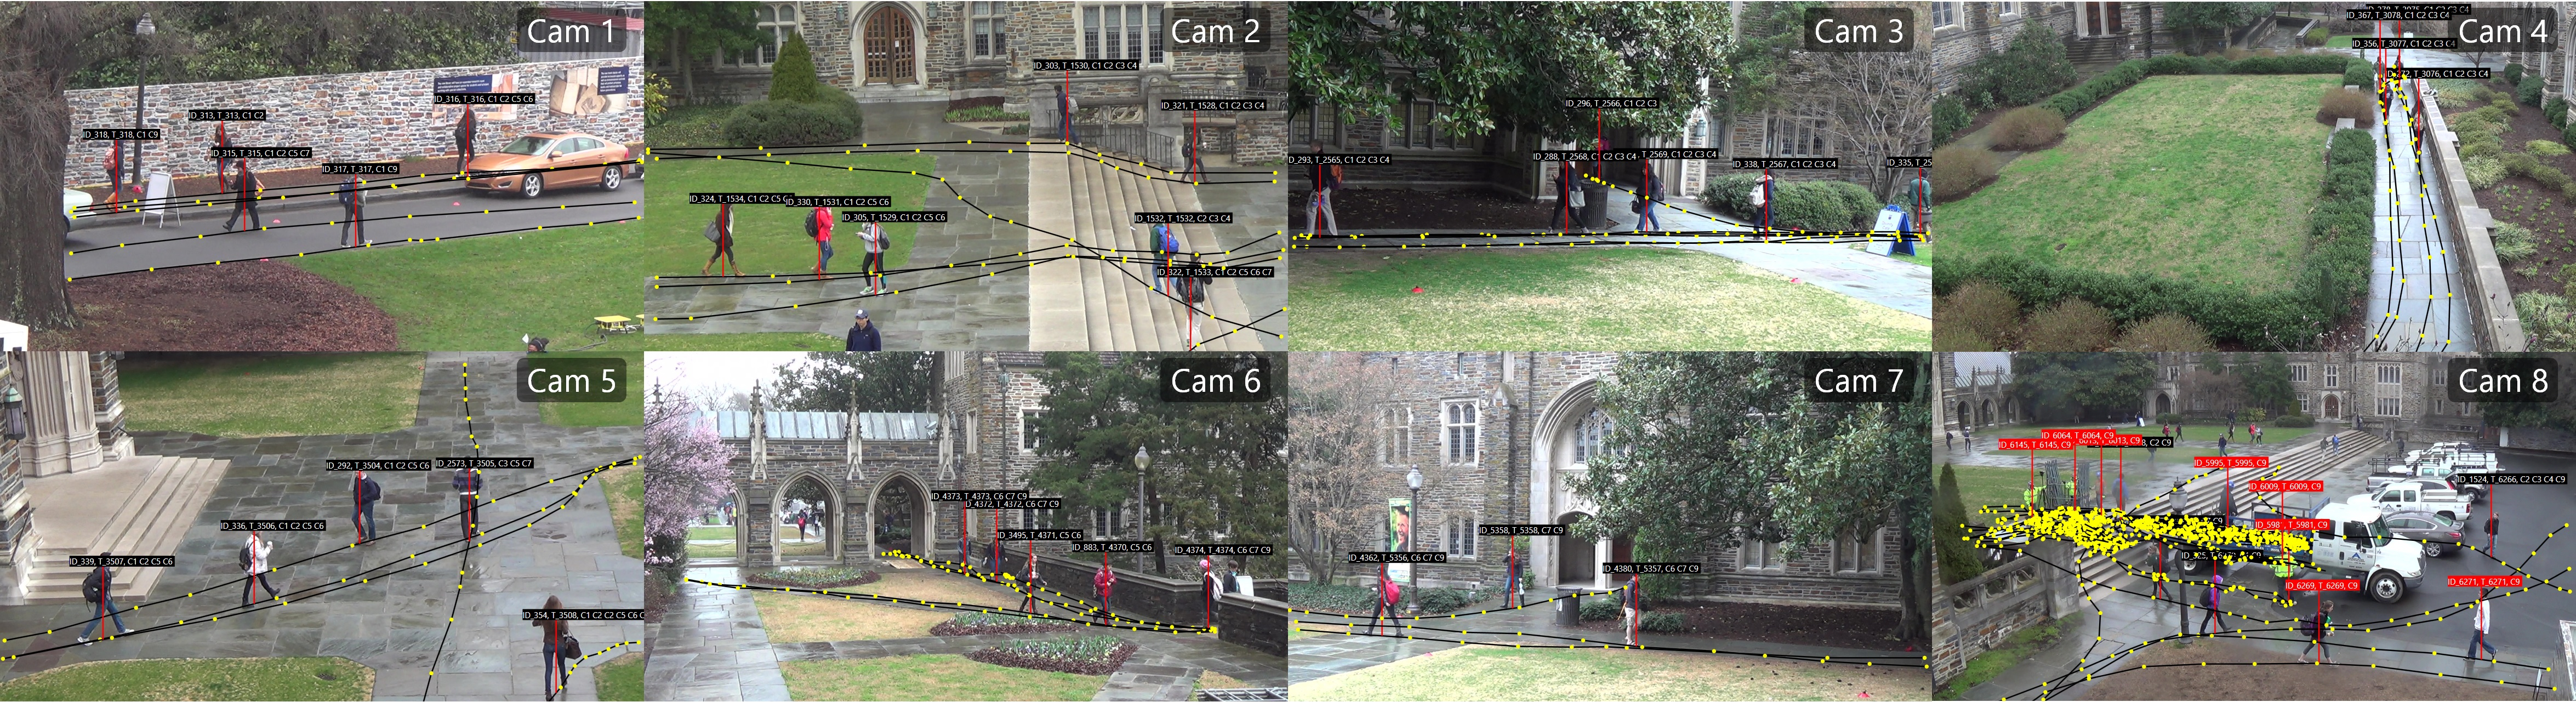
\includegraphics[scale=0.08]{images/duke.jpg}   
\caption{\label{fig:duke} DukeMTMC is a new, manually annotated, calibrated, multi-camera data set recorded outdoors on the Duke University campus \cite{dukeImg}}
\end{figure}
%%%%%%%%%% IMAGES (end) %%%%%%%%%%%%%

Features for Multi-Target Multi-Camera Tracking and Re-Identification \cite{MTMCReID}, is a paper developed by the a group of researchers from Duke University in United States about tracking many people through video taken from several cameras.\\

Their algorithm  learns features using an adaptive weighted triplet and 
assigns adaptive weights using the soft-max/min distribution. Finally an identity label is assigned to the detected observations (people).
The model is trained using an ImageNet network pretrained using data augmentation. Trajectories are computed online in a sliding window,  finally the ones with low confidence are removed. \\

The authors run different experiments, including: 

\begin{itemize}
\item Measure overall MTMCT performance.
\item Measure the impact of improved detector and features during tracking.
\item Study the relation between measures of accuracy. 
\item Demonstrate the usefulness of the methods used.
\item Analyze tracker failures.
\end{itemize}

We tried to understand the paper and apply the same solution to cars but we didn't succeed because some details were difficult to understand. In addition, we don't know the trajectories in advance and this is an input needed. But, what made us give up with this paper was the fact that training the network, as they explain in the paper, was very cost expensive and we were not able to make Google Cloud \cite{GoogleCloud} work in previous weeks.  



\section{MCMT II WORKSHOP AND CHALLENGE}
\label{sec:MTMC_Workshop}
Regarding the previous section, we found a code in Matlab uploaded in a github repository \cite{DeepCC}. The code follows the steps described in section \ref{sec:MTMC_ReID}. 
It is the code of the PhD disertation from Ergys Ristani who also participates in the motchallenge \cite{Motchallenge} providing technical support. This challenge pretends to pave the way for a unified framework towards more meaningful quantification of multi-target tracking.  This objective is similar to the Nvidia Challange, but they focus in people instead of vehicles.\\
We spent a couple of hours trying to understand what he does and testing with our video but the results were awful with the pretrained weights.

%%%%%%%%%% IMAGES %%%%%%%%%%%%%
\begin{figure}[ht] \centering
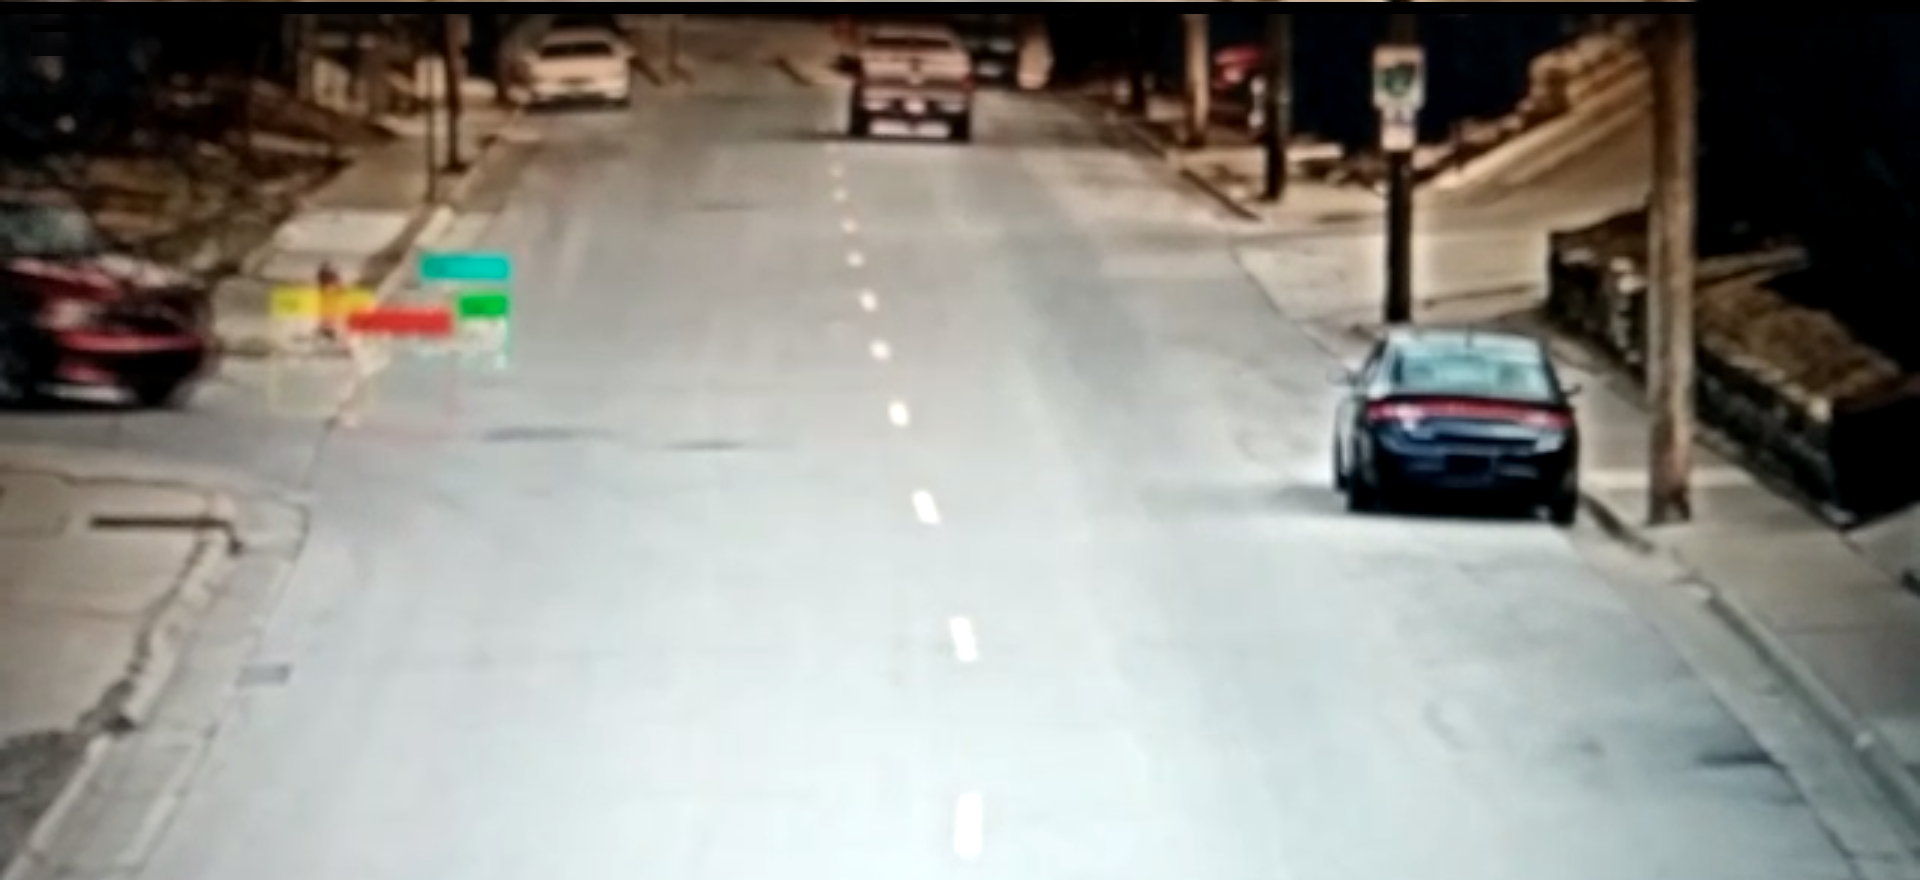
\includegraphics[scale=0.2]{images/bad_results.png}   
\caption{\label{fig:dadRes} II Workshop and Challenge, code tested over our video.  False detections are observed at the left of the images}
\end{figure}
%%%%%%%%%% IMAGES (end) %%%%%%%%%%%%%

Finally we discarded this algorithm because to understand it completely download ~160 GB of data was needed.

\bibliographystyle{IEEEbib}
\bibliography{bibliography}

\end{document}